\section{Horizon Length}

In order to determine what horizon length is needed to optimize the path, several paths were optimized with horizon lengths varying from $10$ to $140$ spaced by $10$. The different horizon lengths were used to optimize a path consisting of a $45\degree$ turn, and both linear and curved paths were used. The results of these optimizations can be seen in Figures \ref{fig:lin_45deg_uav_position} to \ref{fig:cur_45deg_150m_camera_position}.

The results for the three paths are very similar; the longer horizon length, the better tracking of the path. The MPC starts turning earlier than the ground track to compensate for the shift in the camera position, and the aircraft straightens out from the turn later for the same reason.

For the shorter horizon lengths the MPC runs into problems because it hasn't planned far enough ahead when the turn begins. Since it does not look far into the future the aircraft is stille straight above the path when the turn begins. At that point it is too late to start altering the aircrafts position to ensure that the camera stays on the path, so the MPC uses a roll angle in the opposite direction to keep observing the path. This in turn leads to the aircraft turning left, worsening the situation and making the problem more and more difficult. In some cases this causes the roll angle to become very high, causing the MPC to lose control and the aircraft loses height.

Upon closer inspections it can be seen that when the horizon length reaches $90$, there are no more big unwanted motions in the system. As the horizon length reaches $110$ the optimized paths are almost identical, but lincreasing the horizon length still increases the accuracy of the path tracking. The optimization is time consuming, and the duration it takes to optimize the paths increases exponentially. For this reason a horizon length of $110$ will be used for the rest of the simulations, since this gives a accurate path tracking for a relatively short computation time.

%% Position figures
\begin{figure}
	\centering
    \makebox[\textwidth][c]{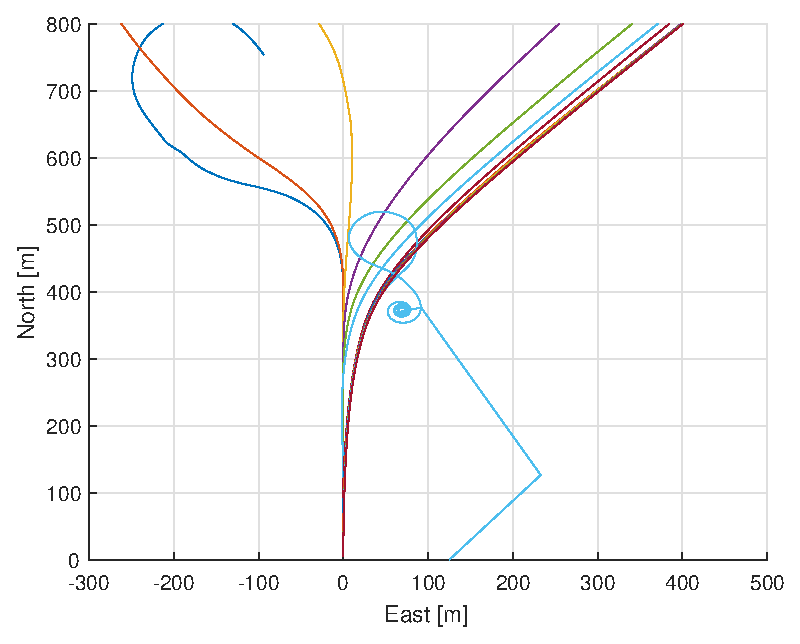
\includegraphics[width=0.8\textwidth, keepaspectratio=true]{../../results/opt/horizon/lin_45deg/fig/uav_position.eps}}
	\caption{Position of the UAV with different horizon lengths when tracking a $45\degree$ turn.}
	\label{fig:lin_45deg_uav_position}
\end{figure}

\begin{figure}
	\centering
    \makebox[\textwidth][c]{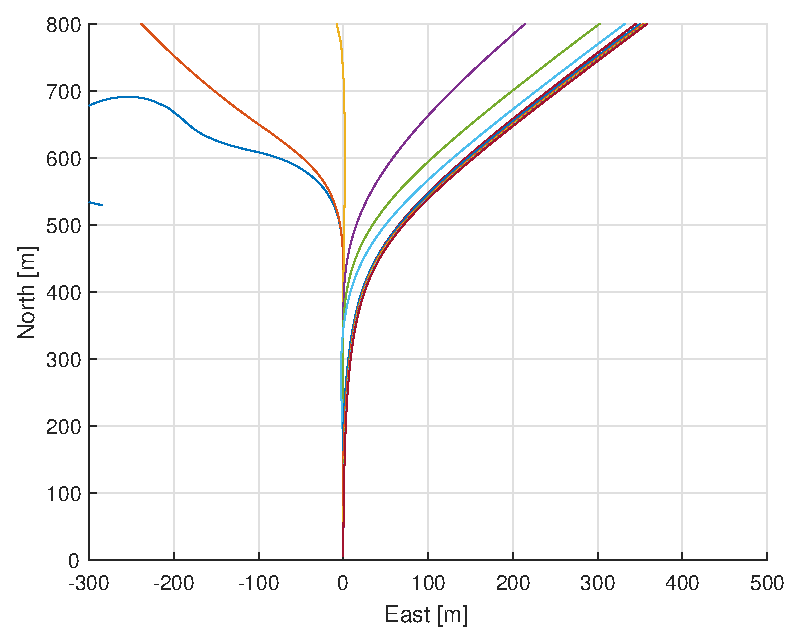
\includegraphics[width=0.8\textwidth, keepaspectratio=true]{../../results/opt/horizon/cur_45deg_200m/fig/uav_position.eps}}
	\caption{Position of the UAV with different horizon lengths when tracking a $45\degree$ turn with $200$ m radius.}
	\label{fig:cur_45deg_200m_uav_position}
\end{figure}

\begin{figure}
	%% This file was created by matlab2tikz.
%
%The latest updates can be retrieved from
%  http://www.mathworks.com/matlabcentral/fileexchange/22022-matlab2tikz-matlab2tikz
%where you can also make suggestions and rate matlab2tikz.
%
\definecolor{mycolor1}{rgb}{0.00000,0.44700,0.74100}%
\definecolor{mycolor2}{rgb}{0.85000,0.32500,0.09800}%
\definecolor{mycolor3}{rgb}{0.92900,0.69400,0.12500}%
\definecolor{mycolor4}{rgb}{0.49400,0.18400,0.55600}%
\definecolor{mycolor5}{rgb}{0.46600,0.67400,0.18800}%
\definecolor{mycolor6}{rgb}{0.30100,0.74500,0.93300}%
\definecolor{mycolor7}{rgb}{0.63500,0.07800,0.18400}%
%
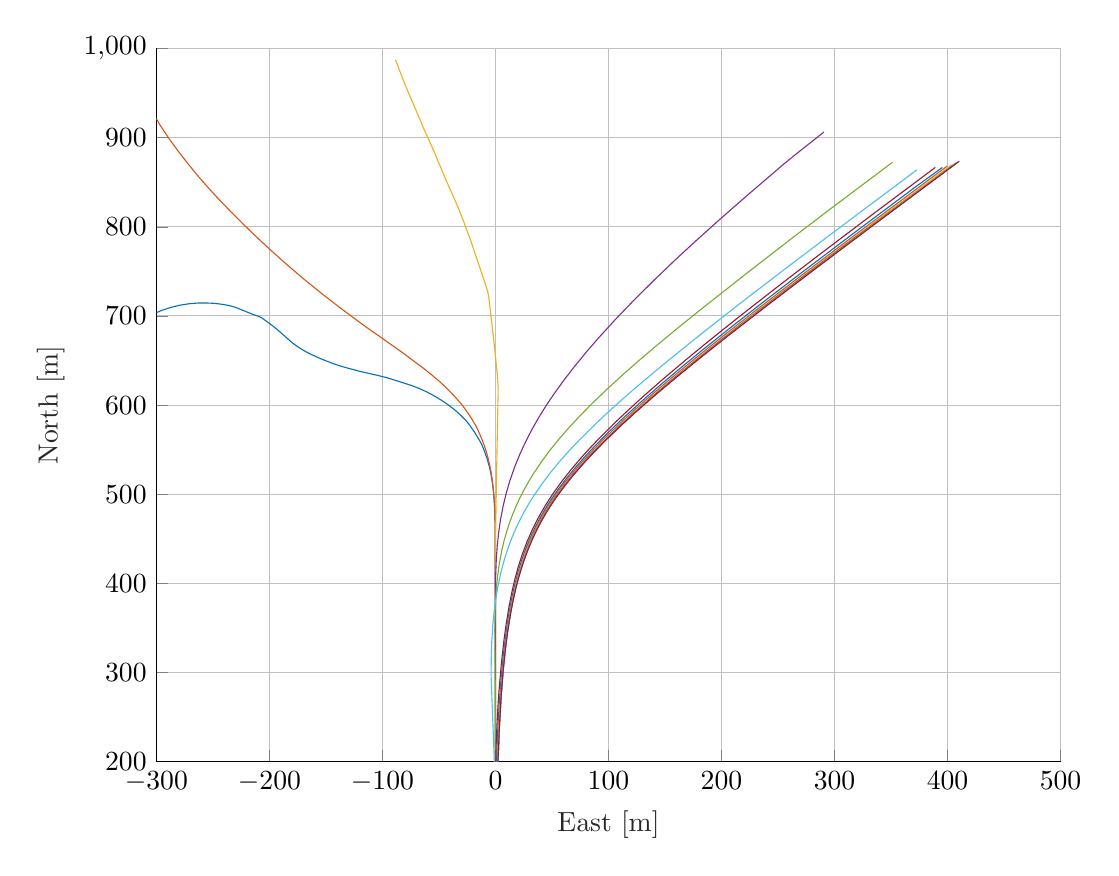
\begin{tikzpicture}

\begin{axis}[%
width=4.521in,
height=3.566in,
at={(0.758in,0.481in)},
scale only axis,
xmin=-300,
xmax=500,
xlabel style={font=\color{white!15!black}},
xlabel={East [m]},
ymin=200,
ymax=1000,
ylabel style={font=\color{white!15!black}},
ylabel={North [m]},
axis background/.style={fill=white},
axis x line*=bottom,
axis y line*=left,
xmajorgrids,
ymajorgrids
]
\addplot [color=mycolor1, forget plot]
  table[row sep=crcr]{%
0	199.711\\
-0.198477000000025	464.619\\
-0.704311999999959	484.74\\
-1.50747000000001	499.845\\
-2.37644999999998	509.911\\
-3.56962999999996	519.978\\
-5.19245000000001	530.014\\
-7.43439000000001	540.034\\
-10.208	550.011\\
-11.8859	554.955\\
-13.8431	559.862\\
-18.4481	569.589\\
-23.7934	579.117\\
-26.9054	583.725\\
-30.3775000000001	588.21\\
-34.1632	592.575\\
-38.2062	596.811\\
-42.4789	600.904\\
-47.0139	604.813\\
-51.7958	608.542\\
-56.7854	612.106\\
-61.9735000000001	615.466\\
-67.3602	618.567\\
-72.9617	621.338\\
-84.593	626.215\\
-96.4595	630.81\\
-102.465	632.768\\
-120.408	637.962\\
-132.1	641.958\\
-137.756	644.042\\
-143.212	646.336\\
-153.673	651.524\\
-163.57	657.117\\
-168.117	660.161\\
-172.361	663.375\\
-176.308	666.692\\
-179.906	670.065\\
-186.083	676.884\\
-191.838	683.448\\
-197.251	689.009\\
-206.453	697.619\\
-208.519	699.058\\
-212.948	701.047\\
-215.489	702.173\\
-229.647	709.49\\
-233.957	711.078\\
-238.571	712.372\\
-243.718	713.394\\
-249.548	714.162\\
-256.127	714.569\\
-263.351	714.458\\
-270.986	713.692\\
-278.814	712.133\\
-286.626	709.799\\
-294.3	706.678\\
-301.797	702.784\\
};
\addplot [color=mycolor2, forget plot]
  table[row sep=crcr]{%
0	199.699\\
-0.190883999999983	464.305\\
-0.669324999999958	484.197\\
-1.38932	499.07\\
-2.60393999999997	513.874\\
-3.71405000000004	523.69\\
-5.20420999999999	533.436\\
-7.07195000000002	543.122\\
-9.32019000000003	552.705\\
-12.1424	562.158\\
-15.3138	571.509\\
-17.0654	576.107\\
-21.2172	585.072\\
-25.8988000000001	593.889\\
-31.0103	602.494\\
-36.9171	610.768\\
-43.1694	618.951\\
-49.8404	626.88\\
-57.0055	634.514\\
-64.4462	641.996\\
-84.0673	660.511\\
-117.12	689.99\\
-137.709	709.37\\
-153.988	725.357\\
-169.908	741.74\\
-185.386	758.519\\
-200.475	775.664\\
-215.195	793.144\\
-229.543	810.997\\
-243.488	829.178\\
-253.491	842.873\\
-263.038	856.801\\
-272.216	870.946\\
-280.914	885.241\\
-289.229	899.643\\
-296.84	914.193\\
-301.273	923.948\\
};
\addplot [color=mycolor3, forget plot]
  table[row sep=crcr]{%
0	195.188\\
0.218475000000012	460.424\\
0.946323000000007	519.893\\
2.43430999999998	618.586\\
1.65698999999995	633.49\\
-0.608969999999999	662.905\\
-5.86103000000003	720.681\\
-6.53688	725.426\\
-7.49787000000003	730.128\\
-22.2995	786.203\\
-28.9726000000001	808.77\\
-34.7893	826.873\\
-45.2617	856.853\\
-55.4231	887.696\\
-62.5049	907.442\\
-80.7313	961.732\\
-88.3607	987.141\\
};
\addplot [color=mycolor4, forget plot]
  table[row sep=crcr]{%
0	195.964\\
0.145627999999988	407.107\\
0.750937000000022	427.084\\
1.57687999999996	442.037\\
2.82623999999998	456.951\\
4.53188	471.809\\
6.78467000000001	486.593\\
9.57241999999997	501.274\\
12.9353	515.828\\
16.9127999999999	530.224\\
21.4375	544.456\\
26.5489	558.501\\
32.1665	572.351\\
38.2773	586.003\\
44.8727	599.433\\
51.8618	612.666\\
61.7945	629.994\\
69.6369	642.771\\
80.4588	659.572\\
91.7284	676.068\\
106.336	696.321\\
121.415	716.201\\
140.005	739.692\\
159.027	762.801\\
178.476	785.544\\
198.243	808.016\\
221.604	833.967\\
255.363	870.669\\
265.865	881.449\\
290.601	906.265\\
};
\addplot [color=mycolor5, forget plot]
  table[row sep=crcr]{%
-2.82281996533129e-06	196.832\\
-0.199991999999952	287.921\\
-0.601101999999969	348.352\\
-0.170873000000029	373.416\\
0.751230999999962	393.413\\
1.91399999999999	408.363\\
3.55934999999999	423.252\\
5.80760999999995	438.055\\
7.65697	447.861\\
9.81444999999997	457.601\\
12.2711	467.267\\
15.0545	476.843\\
18.1507	486.322\\
21.5607	495.693\\
25.2904	504.942\\
29.3101	514.07\\
33.6338	523.061\\
40.6177	536.3\\
48.171	549.226\\
56.2069	561.859\\
64.6873000000001	574.206\\
73.5385	586.296\\
85.7934	602.086\\
98.4779	617.531\\
111.501	632.684\\
124.787	647.593\\
141.719	665.916\\
162.39	687.566\\
183.348	708.93\\
222.181	747.72\\
264.907	789.66\\
297.211	820.826\\
351.38	872.452\\
};
\addplot [color=mycolor6, forget plot]
  table[row sep=crcr]{%
-0.895664000000011	197.559\\
-3.77395999999999	293.468\\
-3.76090999999997	313.577\\
-3.30111999999997	333.636\\
-2.30341999999996	353.642\\
-1.14646000000005	368.605\\
0.427943000000028	383.518\\
2.45081000000005	398.366\\
4.99167	413.122\\
8.10617999999999	427.753\\
11.8486	442.227\\
14.7313	451.771\\
17.9167	461.22\\
21.4107	470.561\\
25.2105	479.783\\
29.3024	488.879\\
33.687	497.839\\
40.7693	511.017\\
48.4272	523.878\\
56.5755	536.441\\
65.16	548.712\\
74.117	560.717\\
83.3777	572.494\\
96.1167	587.886\\
109.203	602.984\\
122.563	617.834\\
139.58	636.095\\
160.398	657.751\\
185.077	682.834\\
217.135	714.703\\
253.065	749.648\\
296.518	791.395\\
361.96	853.547\\
372.876	863.852\\
};
\addplot [color=mycolor7, forget plot]
  table[row sep=crcr]{%
0.258001000000036	197.854\\
0.711377999999968	223.138\\
1.78662999999995	253.357\\
3.07240999999999	278.516\\
5.13156000000004	308.666\\
7.28340000000003	333.661\\
9.39124000000004	353.583\\
11.9341000000001	373.425\\
14.2002	388.239\\
16.8486	402.973\\
19.9557	417.601\\
23.6054	432.092\\
27.8543	446.415\\
32.74	460.534\\
36.3616	469.815\\
40.2735	478.979\\
44.4684999999999	488.019\\
51.2805	501.332\\
58.6683	514.345\\
66.5689	527.071\\
74.9047	539.53\\
83.6067	551.744\\
92.6286	563.736\\
105.11	579.485\\
117.992	594.955\\
131.172	610.141\\
148.068	628.895\\
168.774	651.071\\
189.819	672.948\\
214.669	698.135\\
247.012	730.208\\
283.23	765.501\\
330.58	810.949\\
389.196	866.613\\
};
\addplot [color=mycolor1, forget plot]
  table[row sep=crcr]{%
0.950555000000008	197.999\\
1.81023000000005	228.318\\
3.30048999999997	263.569\\
5.04179999999997	293.691\\
6.91467	318.732\\
9.26084000000003	343.678\\
11.5877	363.553\\
14.4351	383.333\\
16.995	398.083\\
19.9982	412.733\\
23.5323	427.251\\
27.6641	441.606\\
32.4363	455.762\\
35.9814	465.071\\
39.8209000000001	474.264\\
43.9479	483.334\\
48.3577	492.273\\
55.4748	505.428\\
63.1485	518.28\\
71.3054	530.847\\
79.8808	543.154\\
88.8304000000001	555.264\\
101.264	571.143\\
114.203	586.784\\
127.445	602.096\\
144.405	620.927\\
161.714	639.475\\
182.83	661.431\\
207.835	686.743\\
236.76	715.387\\
273.282	750.913\\
321.173	796.838\\
372.95	845.938\\
395.429	866.568\\
};
\addplot [color=mycolor2, forget plot]
  table[row sep=crcr]{%
1.65799000000004	198.436\\
3.05106999999998	238.929\\
4.71024999999997	274.212\\
6.59902999999997	304.325\\
8.61461999999995	329.315\\
10.6185	349.237\\
13.0749	369.081\\
15.2848	383.897\\
17.8762	398.637\\
20.9176	413.276\\
24.4932	427.781\\
28.6684	442.119\\
31.8067	451.568\\
35.2359	460.917\\
38.981	470.144\\
43.0537	479.235\\
47.437	488.184\\
54.5093000000001	501.359\\
62.1511	514.257\\
70.3024	526.889\\
78.8968	539.29\\
87.8524	551.457\\
97.1127	563.407\\
109.911	579.106\\
123.132	594.564\\
140.118	613.576\\
157.48	632.286\\
178.694	654.423\\
203.852	679.945\\
232.94	708.775\\
269.671	744.501\\
317.884	790.697\\
384.723	853.993\\
399.582	867.994\\
};
\addplot [color=mycolor3, forget plot]
  table[row sep=crcr]{%
1.76259000000005	198.889\\
3.09546	239.372\\
4.73541	274.642\\
6.64248999999995	304.735\\
8.68588	329.712\\
10.7264	349.625\\
13.2261	369.459\\
15.4714	384.267\\
18.1015	398.996\\
21.1865	413.622\\
24.8355	428.104\\
27.6227	437.66\\
30.7087	447.124\\
34.0997	456.484\\
37.7958	465.73\\
41.7914	474.853\\
46.0813000000001	483.845\\
50.6662	492.695\\
58.0673	505.704\\
66.0591000000001	518.497\\
74.5252	531.063\\
83.4229	543.43\\
92.6527	555.572\\
105.391	571.467\\
118.566	587.101\\
132.108	602.518\\
149.42	621.505\\
167.076	640.24\\
188.613	662.459\\
213.943	687.95\\
246.933	720.437\\
287.608	759.772\\
339.781	809.532\\
396.078	862.31\\
403.593	869.372\\
};
\addplot [color=mycolor4, forget plot]
  table[row sep=crcr]{%
2.24071000000004	198.955\\
3.50112999999999	239.415\\
5.08487000000002	274.665\\
6.93520999999998	304.816\\
8.96532000000002	329.823\\
11.0376	349.748\\
13.5977	369.586\\
15.9059999999999	384.39\\
18.6145	399.11\\
21.7914	413.721\\
25.4952	428.195\\
29.7806	442.503\\
33.0026	451.926\\
36.5254	461.241\\
40.3615	470.44\\
44.5077	479.513\\
48.9491	488.45\\
53.6661	497.245\\
61.2445	510.187\\
69.4376	522.968\\
78.0652	535.481\\
87.0454	547.727\\
96.3963	559.821\\
109.318	575.688\\
122.663	591.291\\
139.826	610.488\\
157.384	629.384\\
178.857	651.755\\
204.269	677.49\\
233.665	706.577\\
270.806	742.644\\
312.023	782.076\\
357.297	824.577\\
406.4	870.568\\
};
\addplot [color=mycolor5, forget plot]
  table[row sep=crcr]{%
2.20955000000004	199.133\\
3.46844999999996	239.728\\
5.04713000000004	275.077\\
6.57555000000002	300.194\\
8.55393000000004	325.205\\
10.5489	345.138\\
13.0027	364.991\\
15.2092	379.814\\
17.7915	394.56\\
20.8131	409.206\\
24.357	423.72\\
28.499	438.067\\
31.6202	447.52\\
35.04	456.871\\
38.7603	466.109\\
42.7818	475.223\\
47.0974	484.211\\
51.7204	493.097\\
59.1772	506.186\\
67.2035	519.015\\
75.7044	531.589\\
84.6653	543.992\\
93.9602	556.168\\
106.797	572.094\\
120.102	587.778\\
133.775	603.235\\
151.25	622.262\\
172.623	644.723\\
197.991	670.568\\
227.366	699.75\\
264.507	735.906\\
309.421	778.958\\
373.4	839.59\\
407.45	871.541\\
};
\addplot [color=mycolor6, forget plot]
  table[row sep=crcr]{%
2.21456000000001	199.34\\
3.49906999999996	239.952\\
4.84869000000003	270.269\\
6.68430000000001	300.486\\
8.69146000000001	325.522\\
10.7149000000001	345.461\\
13.202	365.314\\
15.4346	380.134\\
18.0423	394.877\\
21.0823	409.52\\
24.6394	424.031\\
28.7945999999999	438.377\\
31.9197	447.831\\
35.3368	457.185\\
39.0513	466.43\\
43.0739	475.555\\
47.3924	484.551\\
51.9997	493.421\\
59.4181	506.475\\
67.4338	519.303\\
75.9449	531.889\\
84.8918	544.264\\
94.2093	556.445\\
107.139	572.44\\
120.51	588.148\\
134.247	603.623\\
151.812	622.679\\
169.687	641.422\\
195.244	667.412\\
224.804	696.754\\
262.168	733.123\\
310.867	779.79\\
371.162	836.917\\
408.955	872.427\\
};
\addplot [color=mycolor7, forget plot]
  table[row sep=crcr]{%
2.20725000000004	199.486\\
3.51845000000003	240.103\\
4.89274	270.42\\
6.71991000000003	300.571\\
8.74310000000003	325.577\\
10.7808	345.502\\
13.2849	365.346\\
15.5316	380.16\\
18.1547	394.896\\
21.2186	409.533\\
24.8004	424.038\\
28.9752999999999	438.376\\
33.7757	452.517\\
37.3296	461.822\\
41.1882000000001	471.023\\
45.3483	480.105\\
49.8081	489.074\\
54.5701	497.934\\
62.2148	510.964\\
70.3967	523.706\\
79.062	536.224\\
88.1651000000001	548.56\\
97.6422	560.728\\
110.741	576.678\\
124.265	592.327\\
141.602	611.531\\
159.474	630.568\\
181.193	652.958\\
206.916	678.805\\
240.403	711.736\\
281.703	751.637\\
334.622	802.086\\
399.028	862.855\\
410.388	873.544\\
};
\end{axis}
\end{tikzpicture}%
	\centering
    \makebox[\textwidth][c]{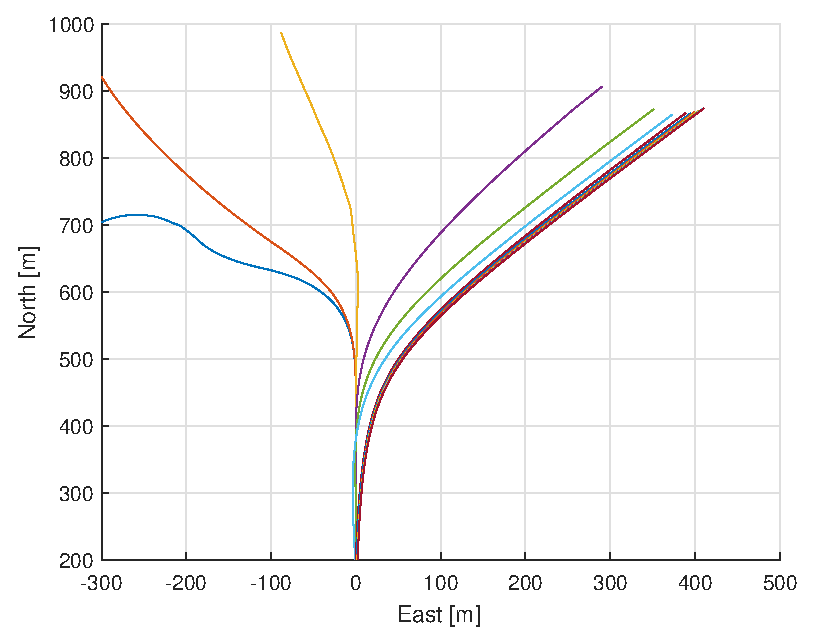
\includegraphics[width=0.8\textwidth, keepaspectratio=true]{../../results/opt/horizon/cur_45deg_150m/fig/uav_position.eps}}
	\caption{Position of the UAV with different horizon lengths when tracking a $45\degree$ turn with $150$m radius.}
	\label{fig:cur_45deg_150m_uav_position}
\end{figure}


%% Camera position
\begin{figure}
	\centering
    \makebox[\textwidth][c]{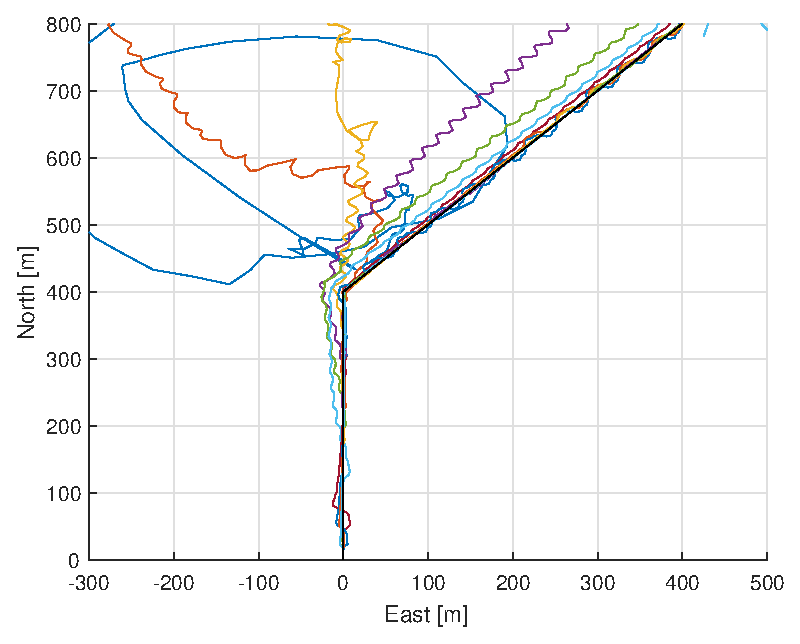
\includegraphics[width=0.8\textwidth, keepaspectratio=true]{../../results/opt/horizon/lin_45deg/fig/camera_position.eps}}
	\caption{Position of the camera centre point with different horizon lengths when tracking a $45\degree$ turn.}
	\label{fig:lin_45deg_camera_position}
\end{figure}

\begin{figure}
	\centering
    \makebox[\textwidth][c]{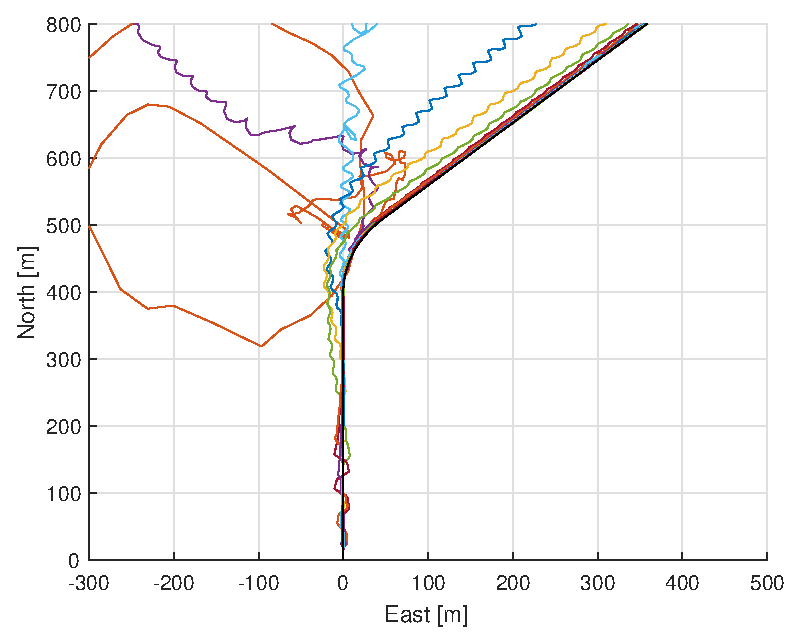
\includegraphics[width=0.8\textwidth, keepaspectratio=true]{../../results/opt/horizon/cur_45deg_200m/fig/camera_position.eps}}
	\caption{Position of the camera centre point with different horizon lengths when tracking a $45\degree$ turn with $200$m radius.}
	\label{fig:cur_45deg_200m_camera_position}
\end{figure}

\begin{figure}
	\centering
    \makebox[\textwidth][c]{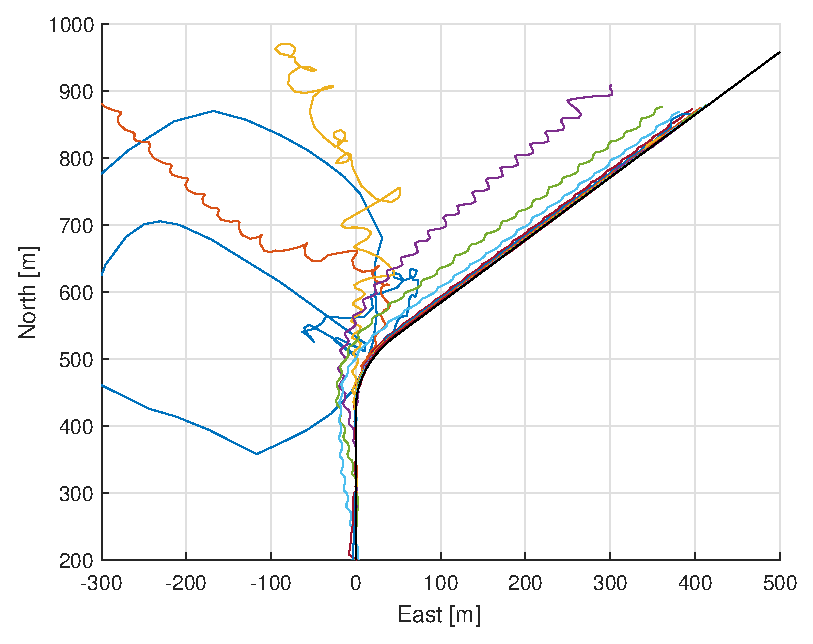
\includegraphics[width=0.8\textwidth, keepaspectratio=true]{../../results/opt/horizon/cur_45deg_150m/fig/camera_position.eps}}
	\caption{Position of the camera centre point with different horizon lengths when tracking a $45\degree$ turn with $150$m radius.}
	\label{fig:cur_45deg_150m_camera_position}
\end{figure}


%% Height
%\begin{figure}
%	\centering
%    \makebox[\textwidth][c]{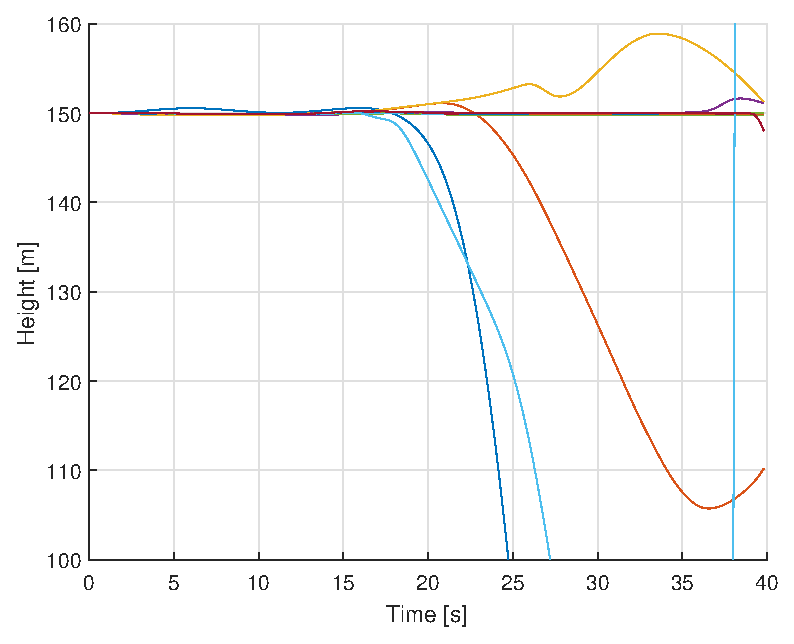
\includegraphics[width=0.8\textwidth, keepaspectratio=true]{../../results/opt/horizon/lin_45deg/fig/height.eps}}
%	\caption{Height of the UAV with different horizon lengths when tracking a $45\degree$ turn.}
%	\label{fig:lin_45deg_height}
%\end{figure}

%\begin{figure}
%	\centering
%    \makebox[\textwidth][c]{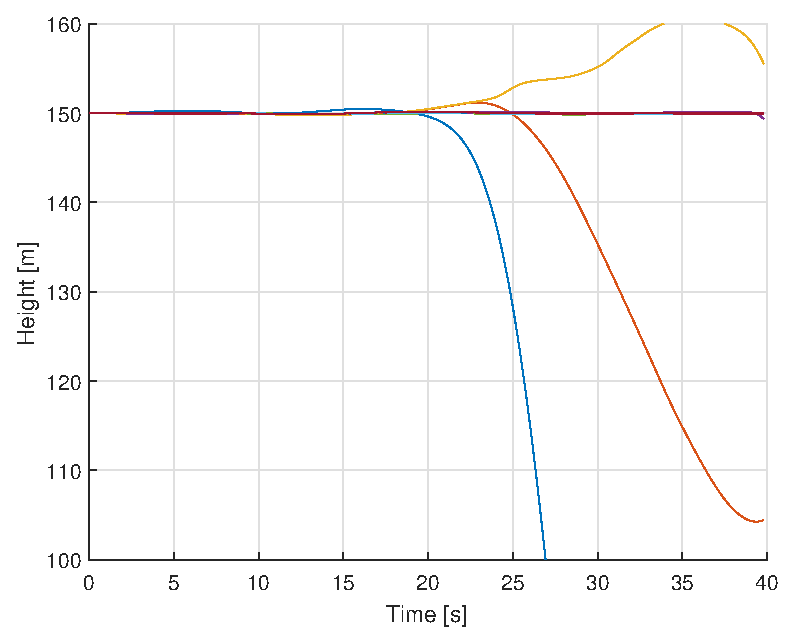
\includegraphics[width=0.8\textwidth, keepaspectratio=true]{../../results/opt/horizon/cur_45deg_200m/fig/height.eps}}
%	\caption{Height of the UAV with different horizon lengths when tracking a $45\degree$ turn with $200$m radius.}
%	\label{fig:cur_45deg_200m_height}
%\end{figure}

%\begin{figure}
%	\centering
%    \makebox[\textwidth][c]{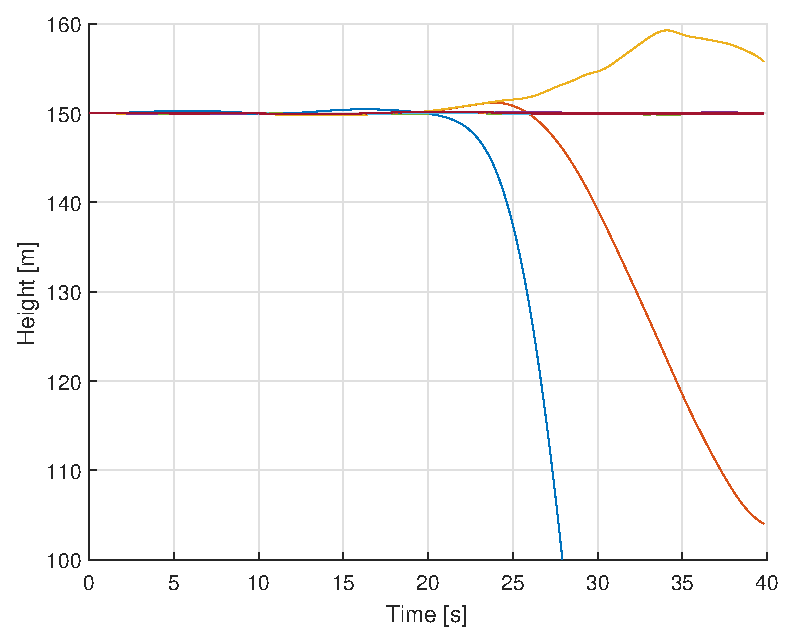
\includegraphics[width=0.8\textwidth, keepaspectratio=true]{../../results/opt/horizon/cur_45deg_150m/fig/height.eps}}
%	\caption{Height of the UAV with different horizon lengths when tracking a $45\degree$ turn with $150$m radius.}
%	\label{fig:cur_45deg_150m_height}
%\end{figure}


%% Attitude
%\begin{figure}
%	\centering
%    \makebox[\textwidth][c]{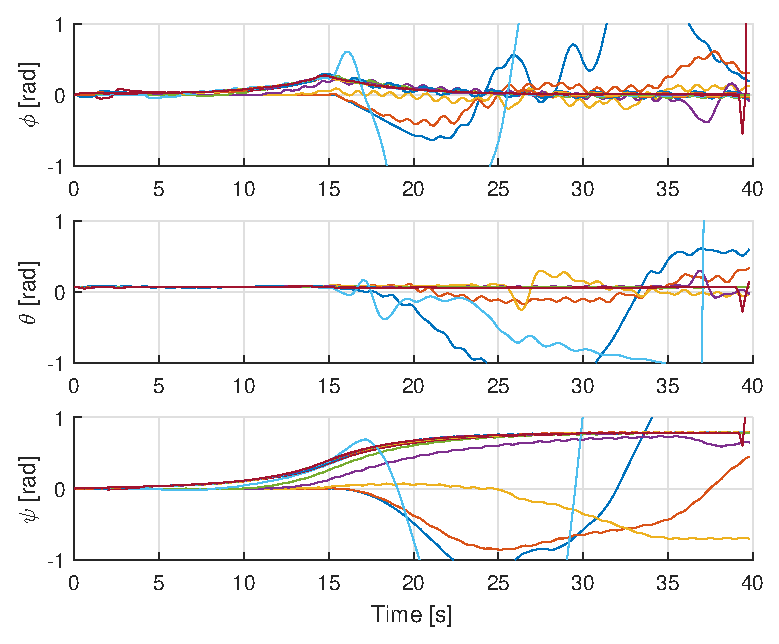
\includegraphics[width=0.8\textwidth, keepaspectratio=true]{../../results/opt/horizon/lin_45deg/fig/attitude.eps}}
%	\caption{Attitude of the UAV with different horizon lengths when tracking a $45\degree$ turn.}
%	\label{fig:lin_45deg_attitude}
%\end{figure}

%\begin{figure}
%	\centering
%    \makebox[\textwidth][c]{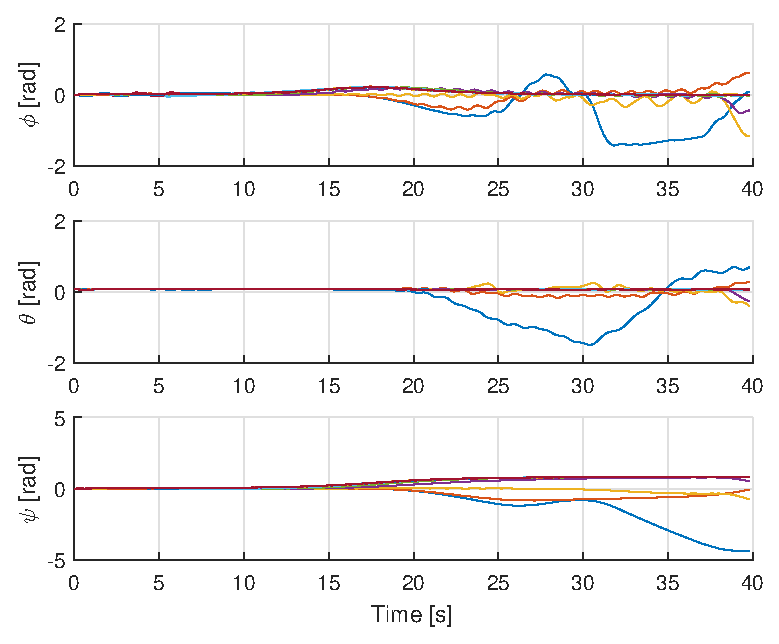
\includegraphics[width=0.8\textwidth, keepaspectratio=true]{../../results/opt/horizon/cur_45deg_200m/fig/attitude.eps}}
%	\caption{Attitude of the UAV with different horizon lengths when tracking a $45\degree$ turn with $200$m radius.}
%	\label{fig:cur_45deg_200m_attitude}
%\end{figure}

%\begin{figure}
%	\centering
 %   \makebox[\textwidth][c]{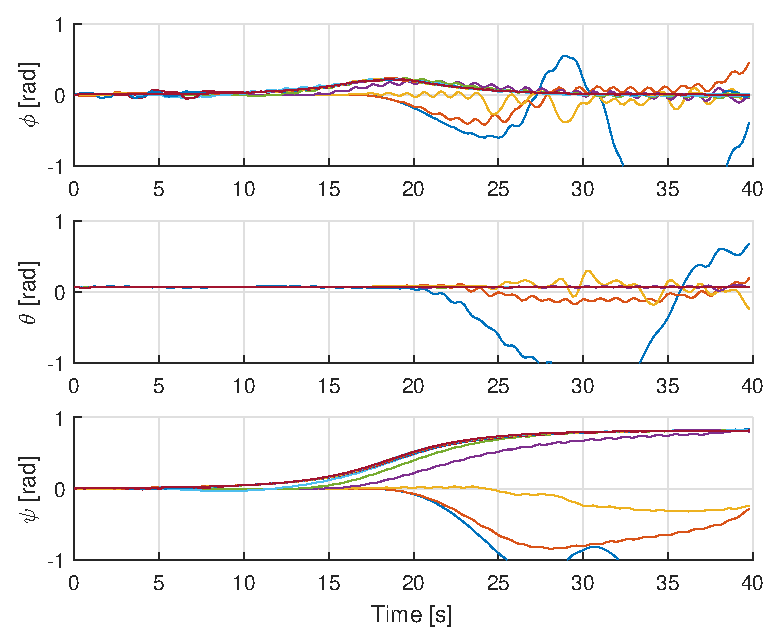
\includegraphics[width=0.8\textwidth, keepaspectratio=true]{../../results/opt/horizon/cur_45deg_150m/fig/attitude.eps}}
%	\caption{Attitude of the UAV with different horizon lengths when tracking a $45\degree$ turn with $150$m radius.}
%	\label{fig:cur_45deg_150m_attitude}
%\end{figure}